\subsubsection{Results}

Results for GMM are calculated the same way as for k-means. The only difference is the function that we are using in order to generate the model.
\begin{listing}[H]
\caption{Evaluate gmm model}
\begin{minted}{python}
def evaluate_gmm_model(train_df, test_df, max_k, file_Path):
    silhouette_scores = []

    for k in range(2, max_k + 1):
        predictions = create_gmm_model(train_df, test_df, k)

        evaluator = ClusteringEvaluator()

        silhouette = evaluator.evaluate(predictions)

        silhouette_scores.append(silhouette)

    plt.plot(range(2, max_k + 1), silhouette_scores, marker='o')
    plt.xlabel('Number of Clusters (k)')
    plt.ylabel('Silhouette Score')
    plt.title('Silhouette Score vs. Number of Clusters')

    plt.savefig(file_Path)

    plt.close()
\end{minted}
\end{listing}

\begin{figure}[H]
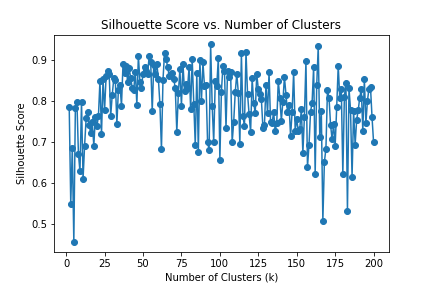
\includegraphics[scale=0.85]{img/Model/Clustering/gmm.png}
\centering
\caption{Silhouette GMM}
\label{fig:SVM_confusion_matrix}
\end{figure}